%%%%%%%%%%%%%%%%%%%%%%%%%%%%%%%%%%%%%%%%%
% Beamer Presentation
% LaTeX Template
% Version 1.0 (10/11/12)
%
% This template has been downloaded from:
% http://www.LaTeXTemplates.com
%
% License:
% CC BY-NC-SA 3.0 (http://creativecommons.org/licenses/by-nc-sa/3.0/)
%
%%%%%%%%%%%%%%%%%%%%%%%%%%%%%%%%%%%%%%%%%

%----------------------------------------------------------------------------------------
%	PACKAGES AND THEMES
%----------------------------------------------------------------------------------------

\documentclass{beamer}
\setbeamertemplate{page number in head/foot}{\insertframenumber /10}
\usepackage{cite}
\usepackage{amsmath,amssymb,amsfonts}
\usepackage{graphicx}
\usepackage{multicol}
\usepackage{caption}
\usepackage{multimedia}
\usepackage{subcaption}
\usepackage{caption}
\usepackage{textcomp}
\usepackage{xcolor}
\usepackage{url}
\usepackage[czech]{babel}
\usepackage{siunitx}

\graphicspath{{./images}}
\usepackage{caption}
\captionsetup[subfigure]{justification=centering} %configure subfigures to use centered captions
\captionsetup[figure*]{justification=centering} %configure subfigures to use centered captions
\mode<presentation> {
% The Beamer class comes with a number of default slide themes
% which change the colors and layouts of slides. Below this is a list
% of all the themes, uncomment each in turn to see what they look like.

%\usetheme{default}
%\usetheme{AnnArbor}
%\usetheme{Antibes}
%\usetheme{Bergen}
%\usetheme{Berkeley}
%\usetheme{Berlin}
%\usetheme{Boadilla}
%\usetheme{CambridgeUS}
%\usetheme{Copenhagen}
%\usetheme{Darmstadt}
%\usetheme{Dresden}
%\usetheme{Frankfurt}
%\usetheme{Goettingen}
%\usetheme{Hannover}
%\usetheme{Ilmenau}
%\usetheme{JuanLesPins}
%\usetheme{Luebeck}
%\usetheme{Madrid}
%\usetheme{Malmoe}
%\usetheme{Marburg}
%\usetheme{Montpellier}
%\usetheme{PaloAlto}
%\usetheme{Pittsburgh}
%\usetheme{Rochester}
%\usetheme{Singapore}
%\usetheme{Szeged}
\usetheme{Warsaw}

% As well as themes, the Beamer class has a number of color themes
% for any slide theme. Uncomment each of these in turn to see how it
% changes the colors of your current slide theme.

%\usecolortheme{albatross}
%\usecolortheme{beaver}
%\usecolortheme{beetle}
%\usecolortheme{crane}
%\usecolortheme{dolphin}
%\usecolortheme{dove}
%\usecolortheme{fly}
%\usecolortheme{lily}
%\usecolortheme{orchid}
%\usecolortheme{rose}
%\usecolortheme{seagull}
%\usecolortheme{seahorse}
%\usecolortheme{whale}
%\usecolortheme{wolverine}

%\setbeamertemplate{footline} % To remove the footer line in all slides uncomment this line
%\setbeamertemplate{footline}[page number] % To replace the footer line in all slides with a simple slide count uncomment this line

%\setbeamertemplate{navigation symbols}{} % To remove the navigation symbols from the bottom of all slides uncomment this line
}

\usepackage{graphicx} % Allows including images
\usepackage{booktabs} % Allows the use of \toprule, \midrule and \bottomrule in tables

%----------------------------------------------------------------
%	TITLE PAGE
%----------------------------------------------------------------

\title[ARI: Stabilizace LEGO segwaye]{Semestrální práce ARI\\ Stabilizace LEGO segwaye} % The short title appears at the bottom of every slide, the full title is only on the title page

\author{Vojtěch Michal -- 
\textit{michavo3@fel.cvut.cz}} % Your name
\date{15. května 2021} 

\begin{document}

\begin{frame}
\titlepage
% Děkuji za slovo. Vážený pane inženýre, vážení kolegové, dovolte mi Vás v krátké prezentaci seznámit s výsledky
% své semestrální práce průběhu MASTER.
\end{frame}

\begin{frame}
% Zadání spočívalo v modelování, analýze a řízení dvoukolového LEGO robota ve snaze udržet jej ve vertikální poloze.
% Je snadné nahlédnout, že se jedná o nestabilní polohu, která vyžaduje aktivní řízení motorků v obou kolech.
    \makebox[\textwidth][c]	{\includegraphics[height=\textheight]{pivo.png}}
\end{frame}


    \begin{frame}
    
        % Matematicky lze segway modelovat jako inverzní kyvadlo s osou otáčení procházející nápravou kol.
        % Kinematiku robota lze popsat dvěma nelineárními diferenciálními rovnicemi parametrizovanými 
        % fyzickými rozměry a rozložením hmoty robota, jakož i elektrickými vlastnostmi baterie a servo motorů.
        % Proměnné veličiny jsou úhel natočení kol \theta a odklon od svislice \psi, obojí v radiánech.
        % Zobecněné síly na pravé straně rovnic jsou závislé na regulovatelném napětí na motorech u ve voltech.

        % S ohledem na fyzikální podstatu odpovídá svislé poloze jako pracovní bod nulový vektor,
        % na jehož okolí jsem aproximoval hodnoty červených nelineárních výrazů v rovnicích.
        
        \frametitle{Matematický model - nelineární ODR}    
        \begin{equation}
            \begin{aligned}
                &\left[(2m + M) R^2 + 2 J_w + 2n^2 J_m\right] \ddot{\theta} + \\
                &+ (MLR \textcolor{red}{\text{cos}\psi} - 2n^2 J_m) \ddot{\psi} - MLR\textcolor{red}{\dot{\psi}^2 \text{sin} \psi} = F_\theta
            \end{aligned}
            \label{eq:pohyb1}
        \end{equation}
        \begin{equation}
            \begin{aligned}
                & (MLR \textcolor{red}{\text{cos} \psi} - 2n^2 J_m) \ddot{\theta} + \\ &+ (ML^2 + J_\psi + 2n^2 J_m) \ddot{\psi}
                - MgL\textcolor{red}{\text{sin}\psi} = F_\psi
            \end{aligned}
            \label{eq:pohyb2}
        \end{equation}
        \begin{equation}
            F_\theta = 2 \alpha u- 2(\beta + f_w) \dot{\theta} + 2\beta\dot{\psi}
            \label{eq:motor1_easy}
        \end{equation}
        \begin{equation}
            F_\psi = - 2 \alpha u + 2\beta \dot{\theta} - 2\beta \dot{\psi}
            \label{eq:motor2_easy}
        \end{equation}

        Požadovaný pracovní bod -- vertikální nestabilní ekvilibrium

        \begin{equation}
            P = \begin{bmatrix}
                \theta_p &    \psi_p &     \dot{\theta}_p &     \dot{\psi}_p & u_p
            \end{bmatrix} = \begin{bmatrix}
                0 & 0 & 0 & 0 & 0
            \end{bmatrix}
            \label{eq:prac_bod}
        \end{equation}
        
    \end{frame}
    
    \begin{frame}
        % Po sestavení jsem měl možnost ověřit přímým měřením hmotnost robota i koleček a dále výšku, šířku a tloušťku robota.
        % Pro účely pozdější analýzy nelinearit jsem se potřeboval seznámit s elektrickými vlastnostmi akumulátoru,
        % jež jsem dopočítal z dvojic (proud, napětí) měřeních při proměnném odebíraném výkonu. 
        % Hodnoty momentů setrvačnosti a vztah pro polohu těžiště byly ponechány z referenčního řešení Yorihisa Yamamoty.
        
        
        \frametitle{Identifikace - parametry}
        
        \begin{figure}[htbp]
            \centerline{\includegraphics[width=\linewidth]{mereni_baterky.jpg}}
            \label{fig:mereni_baterky}        
        \end{figure}
    \end{frame}
    
    \begin{frame}
        % Se známými hodnotami parametrů a zjednodušeními provedenými při linearizaci jsem vyčíslil matematický model
        % pro získání stavového popisu. Zobecnělé souřadnice jsem podle konvence v oboru řízení přeznačil na vektor \vec{x}
        % a dále nalezl Jakobiho matice A, B vyčíslené v pracovním bodě. Pro úplnost jsou uvedeny na slidu se zaokrouhlenými hodnotami prvků. 
        \frametitle{Linearizovaný stavový popis}

        \begin{equation}
            \vec{x} = \begin{bmatrix}
                x_1 \\
                x_2 \\
                x_3 \\
                x_4
            \end{bmatrix} = \begin{bmatrix}
                \theta \\
                \psi \\
                \dot{\theta} \\
                \dot{\psi}
            \end{bmatrix}
        \end{equation}

        \begin{equation}
            \Delta \dot{\vec{x}} = \begin{bmatrix}
                0 &        0 &    1 &        0 \\
                0 &        0 &         0 &   1 \\
                0 &-513 & -204 & 204 \\
                0 & 281 &   85 & -85
            \end{bmatrix} \Delta \vec{x} + \begin{bmatrix}
                0 \\ 0 \\   396 \\-165
            \end{bmatrix} \Delta u
        \end{equation}  

    \end{frame}

    \begin{frame}
        \frametitle{Identifikace - nelinearity}
        % Pro určení věrohodnoti linearizovaného modelu bylo potřeba analyzovat vliv zanedbaných vlastností.

        % Nalezení parametrů Théveninovy náhrady napájení mi umožnilo dopředu odhadnout nejhorší propad napětí pod zátěží
        % a určit tak saturaci akčního zásahu na osm voltů, což následně potvrdil experiment.
        % Pásmo necitlivosti a dynamika motoru byly odečteny z odezvy reálného motoru na různé průběhy řídicího napětí.
        % Protože časové konstanty přechodových dějů v motorech byly méně jak třetinové ve srovnání s vlastní dynamikou inverzního
        % kyvadla, v dalším návrhu řízení jsem je zanedbal.

        % Ze stavových proměnných lze významnou saturaci pozorovat u úhlu náklonu \psi, kde je omezení dáno možností pádu robota na záda.
        % Maximum úhlové rychlost koleček theta dot bylo vypočteno v rámci studia dynamiky motorů.
        \begin{figure}
            \begin{subfigure}{0.45\textwidth}
                \centerline{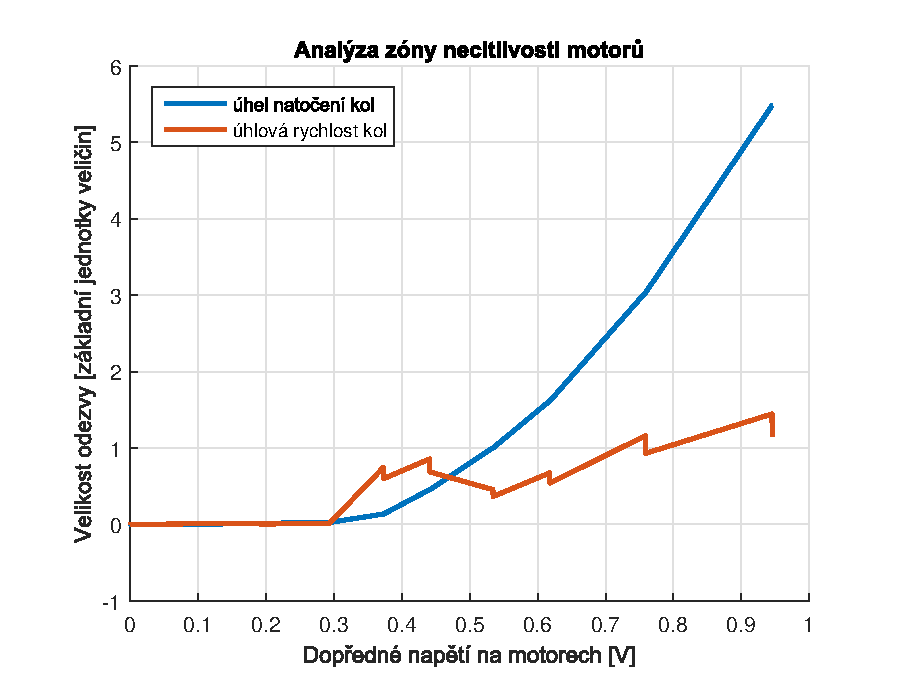
\includegraphics[width=\linewidth]{deadzone_motory_vpred.eps}}
            \end{subfigure}
            \begin{subfigure}{0.45\textwidth}
                \centerline{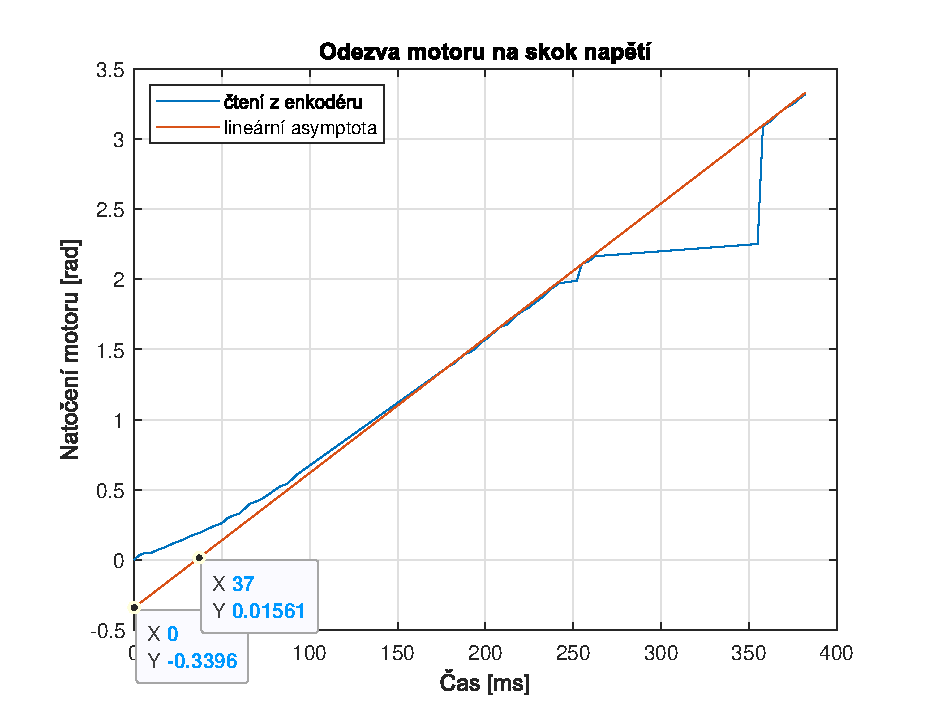
\includegraphics[width=\linewidth]{motor_skok.eps}}
            \end{subfigure}
        \end{figure}
        
        
        \textbf{Saturace akčního zásahu} $\pm 8$ \si{\volt}\\
        \textbf{Pásmo necitlivosti motorů} $\pm 0.3$ \si{\volt}\\        
        \textbf{Dynamika motorů} zanedbatelná \\
        \textbf{Saturace stavů}: \\
        \centering
         $\psi$ v intervalu $\pm \frac{\pi}{2}$ \si{\radian} \\
         $\dot{\theta}$ v intervalu $\pm 16$ \si{\radian\per\second} \\
    
    \end{frame}
    

    \begin{frame}
        % Znalosti nelinearit reálného systému jsem zohlednil v Simulinkovém schématu potřebném pro závěrečné porovnání modelů.
        % Na slidu je vyneseno srovnání odezvy na jednotkový skok akčního zásahu. Je patrné, že linearizace
        % jistou chybu do modelu vnesla, ovšem na okolí pracovního bodu jsou modely velmi shodné. Zejména bych vypíchnul
        % rovnost náklonu \psi obou modelů až do okamžiku saturace
        
        \frametitle{Identifikace - porovnání}
    
        \begin{figure}[htbp]
            \centerline{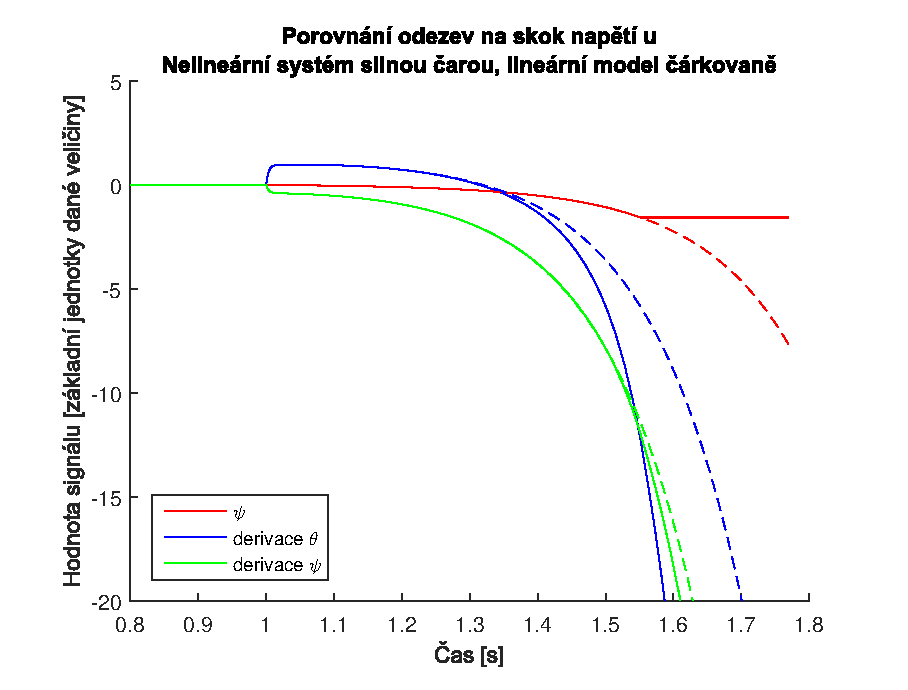
\includegraphics[width=\linewidth]{porovnani_skok.eps}}
            \label{fig:porovnani_skok}        
        \end{figure}
    
    \end{frame}

    \begin{frame}
        % Během návrhu stavové zpětné vazby jsem nalezl tři regulátory.
        % Výstupem první iterace byl regulátor K_1, jehož působení je na videu. Protože byl jeden z pólů uzavřebé smyčky v počátku,
        % nebyl robot schopen se udržet na místě a pomalu couval.

        % Druhá a následně třetí iterace umístily jeden z pólů do bodu -0.5, což se experimentálně projevilo velice pozitivně.
        % I při změně rozložení hmoty přidáním skleněného mlýnku s kořením dokázala SZV dostat systém do klidu.
        % Kompenzace pásma necitlivosti motorů zajistila redukci cukání, díky čemuž mlýnek nespadl i přes velice malou plochu, na které stál.

        
        \frametitle{Balancování stavovou ZV}

        Tři regulátory $K_{1,2,3}$ s rostoucí kvalitou splnění požadavků\\
        
        \begin{figure}[htbp]
            \centerline{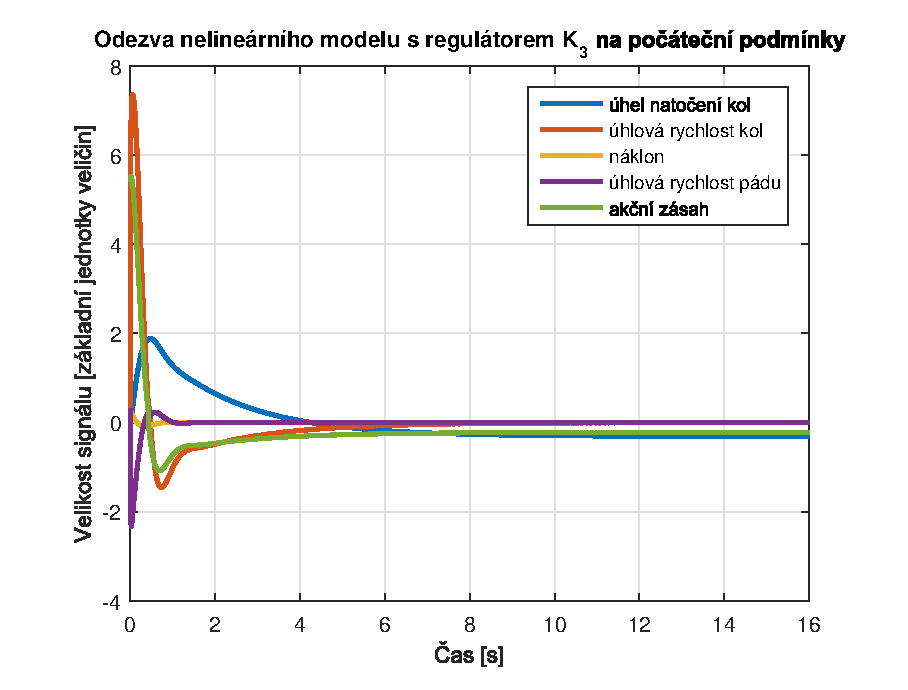
\includegraphics[width=0.6\linewidth]{pp_regulator_K3.eps}}
            \label{fig:porovnani_skok}        
        \end{figure}
        $K_3 \cdots T_s = 1~\si{\second},~OS = 8~\%$. Další dva póly $-231$ a $-0.5$.
    \end{frame}

    \begin{frame}
        % Řízení vzdálenosti od překážky bylo navrhováno tak, aby mohlo využít maximum z kvalitní stavové zpětné vazby.
        % Regulátor vzdálenosti svým výstupem ovlivňoval měření derivace \theta a udával tak rychlost pro posunutí robota.
        % Stavová zpětná vazba následně na svém vstupu přijímala takto pozměněný stav a zajišťovala stabilizaci během přesunu.

        % Protože cílem SZV bylo dosáhnout nulového theta a regulátor vzdálenosti potřeboval theta měnit v zájmu posunu robota na správnou vzdálenost d,
        % měla první iterace řízení problém s omezenými manévrovacími možnostmi, jak je vidět na videu proporcionální regulace.
        % Při posunu robota na nenulovou thetu jsou oba regulátory proti sobě v důsledku čehož se robot přibližně po metru přestane pohybovat.

        \frametitle{Řízení vzdálenosti $d$}

        Rozšíření úlohy balancování o P a PI regulátor vzdálenosti od překážky $d$ měřené ultrazvukovým senzorem. \\
        První nástřel $K_\text{P}$, $K_\text{I}$ výpočtem, dál laděno experimentálně.  
        
        \begin{figure}[htbp]
            \centerline{\includegraphics[width=0.6\linewidth]{proporcionalni_d_experiment.png}}
            \label{fig:porovnani_skok}        
        \end{figure}
    
    \end{frame}

   \begin{frame}
    % Závěrem bych chtěl říci, že modelování i regulace byly úspěšné, ovšem stále existuje prostor pro další zlepšování.
    % Pro přesnější řízení by bylo potřeba ověřit i zbylé konstantní parametry systému a dále opravit částečně nesprávný předpoklad linearizace,
    % že čtverec derivace \psi bude blízký nule. Tímto bych Vám chtěl poděkovat za pozornost a vracím slovo panu inženýrovi.
   \begin{figure}
    \includegraphics[width = \textwidth]{saturace.jpg}
       
   \end{figure}
   \centering
   \textit{Děkuji za pozornost}
   
   \end{frame}
%------------------------------------------------

%------------------------------------------------------------------------------

\end{document}